\documentclass[tikz,border=2pt]{standalone}
\usepackage{amsmath,amssymb}
\usepackage{tikz}
\usetikzlibrary{arrows.meta}

\begin{document}
% Uniform continuity between metric spaces: for a given epsilon, ONE delta works at every
% point of X — each delta-ball is mapped inside the epsilon-ball around the image point.
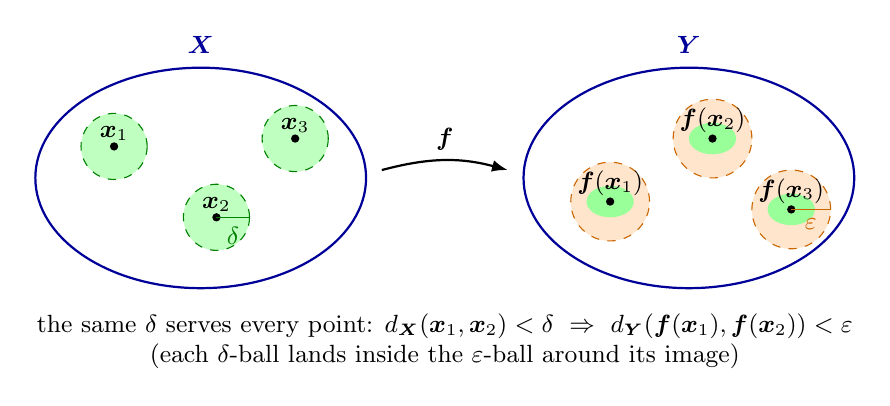
\begin{tikzpicture}[every node/.style={font=\small}, >={Latex[length=2mm]}]
	\draw[thick, blue!60!black] (0,0) ellipse (2.1 and 1.4);
	\node[blue!60!black, anchor=south] at (0,1.45) {$\boldsymbol{X}$};
	\foreach \p/\l in {(-1.1,0.4)/1, (0.2,-0.5)/2, (1.2,0.5)/3} {
		\fill[green!25] \p circle (0.42);
		\draw[green!50!black, dashed] \p circle (0.42);
		\fill \p circle (1.5pt) node[above, inner sep=2pt] {$\boldsymbol{x}_{\l}$};
	}
	\draw[green!50!black] (0.2,-0.5) -- (0.62,-0.5) node[midway, below, font=\small] {$\delta$};
	\draw[->, thick] (2.3,0.1) to[bend left=15] node[above] {$\boldsymbol{f}$} (3.9,0.1);
	\begin{scope}[xshift=6.2cm]
		\draw[thick, blue!60!black] (0,0) ellipse (2.1 and 1.4);
		\node[blue!60!black, anchor=south] at (0,1.45) {$\boldsymbol{Y}$};
		\foreach \p/\l in {(-1.0,-0.3)/1, (0.3,0.5)/2, (1.3,-0.4)/3} {
			\fill[orange!20] \p circle (0.5);
			\draw[orange!80!black, dashed] \p circle (0.5);
			\fill[green!40] \p ellipse (0.3 and 0.2);
			\fill \p circle (1.5pt) node[above, inner sep=2pt] {$\boldsymbol{f}(\boldsymbol{x}_{\l})$};
		}
		\draw[orange!80!black] (1.3,-0.4) -- (1.8,-0.4) node[midway, below, font=\small] {$\varepsilon$};
	\end{scope}
	\node[anchor=north, align=center] at (3.1,-1.6) {the same $\delta$ serves every point: $d_{\boldsymbol{X}}(\boldsymbol{x}_1,\boldsymbol{x}_2)<\delta\ \Rightarrow\ d_{\boldsymbol{Y}}(\boldsymbol{f}(\boldsymbol{x}_1),\boldsymbol{f}(\boldsymbol{x}_2))<\varepsilon$\\ (each $\delta$-ball lands inside the $\varepsilon$-ball around its image)};
\end{tikzpicture}
\end{document}
